\documentclass[11pt,article]{article}
\usepackage[utf8]{inputenc}
\usepackage[T1]{fontenc} % caractères accentués en entrée, dans emacs
\usepackage[french]{babel}
\FrenchFootnotes
\selectlanguage{french}
\usepackage{a4wide} % possibilité d'utiliser toute la page a4
% selon GUT#33, avril 2007, page 13, empagement
% largeur des textes (ou justification) = 15cm
% hauteur du rectangle d'empagement = 23cm
% blanc de couture = 2/5 (21-15) = 2.4 = inner = right
% blanc de grand fond = 3/5 (21-15) = outer = left
% blanc de tête = 2/5 (29,7-23) = top
% blanc de pied = 3/5 (29,7-23) = bottom
%\usepackage[a4paper,twoside=true,right=2.4cm,left=3.6cm,top=2.68cm,bottom=4.02cm]{geometry} 
% selon CFSE 2006
% - largeur des textes (ou justification) : 16cm (2cm de marge, et 1cm
%   de reliure) ;
% - hauteur des textes, y compris les notes : 23cm (2,5cm de marge
%   haute et 2cm de marge basse) ; 1ère page de : 36pts
%   d'espacement avant le titre ;
\oddsidemargin   -4mm           % 3cm a gauche des impaires
\evensidemargin   4mm           % 2cm a gauche des paires
\topmargin       -18mm          % 2.5cm en haut
\headheight       13mm          % taille de l'entete (lignes)
\headsep          24pt          % espace entre entete et texte
\footskip         30pt          % espace entre pied de page et texte
\textheight      230mm          % longeur du texte
\textwidth       160mm          % largeur du texte
\parskip 1pt                    % pas de sauts entre paragraphes
%\parindent 0pt                  % largeur de l'indentation
\usepackage{graphicx} % figure postcript avec latex,
		      % figure png avec pdflatex, au lieu d'utiliser epsfig
\usepackage[usenames,dvipsnames,table]{xcolor}
\usepackage{paralist}
\usepackage{ifthen}
\usepackage{amssymb}
\usepackage{amsfonts}
\usepackage{amsmath}
\usepackage{eurosym}
\usepackage{textcomp}
\usepackage{listings}
\lstset{language=Java,numbers=left,numberstyle=\tiny,stepnumber=4,numbersep=5pt,xleftmargin=5pt}

\usepackage{alltt}
\usepackage{longtable}

% adjust word spacing less strictly
% as result, some spaces between words may be a bit too large,
% but long words will be placed properly.
\sloppy

\newcommand{\cmt}[1]{\texttt{<}\textbf{--~#1~--}\texttt{>}}

\usepackage{lineno}
\usepackage{xspace}

\newcommand{\simint}{\textsc{SimInt}\xspace}

\setlength{\marginparwidth}{1cm}
\setlength{\marginparsep}{10pt}
\reversemarginpar
\newcounter{usecasehaute}
\newcommand{\haute}{Haute}
\newcommand{\moyenne}{Moyenne}
\newcommand{\basse}{basse}
\newcommand{\usecase}[4]{\item \marginpar{\vspace{5pt}\ifthenelse{\equal{#1}{Haute}}{\centering\textsc{#1}\stepcounter{usecasehaute}\newline n$^{\circ}$ \theusecasehaute}{\ifthenelse{\equal{#1}{Moyenne}}{#1}{\small #1}}} #2 \begin{itemize}\item précondition~: #3 \item postcondition~: #4\end{itemize}}
\newcommand{\priorityusecase}[2]{\item \marginpar{\vspace{5pt}\ifthenelse{\equal{#1}{Haute}}{\centering\textsc{#1}\stepcounter{usecasehaute}\newline n$^{\circ}$ \theusecasehaute}{\ifthenelse{\equal{#1}{Moyenne}}{#1}{\small #1}}} #2}
\newcommand{\casusecase}[4]{\usecase{#1}{#2}{#3}{#4}}

\newcommand{\nullvalue}{\textsf{null}\xspace}
\newcommand{\emptyvalue}{\ensuremath\mathrm{vide}}
\newcommand{\invariant}{\ensuremath\mathrm{invariant}}

\begin{document}
\title{Projet CSC4102: Simulation de programmes pour la détection d'interblocage}
\author{Nom Prénom Étudiant1 et Nom Prénom Étudiants2}
\date{Année 2018--2019~---~\today}
\maketitle

\newpage

\tableofcontents

\newpage

\section{Spécification}

\subsection{Diagrammes de cas d'utilisation}

{\color{red}\textbf{Le diagramme suivant est à compléter.}}

\begin{figure}[h!]
\begin{center}
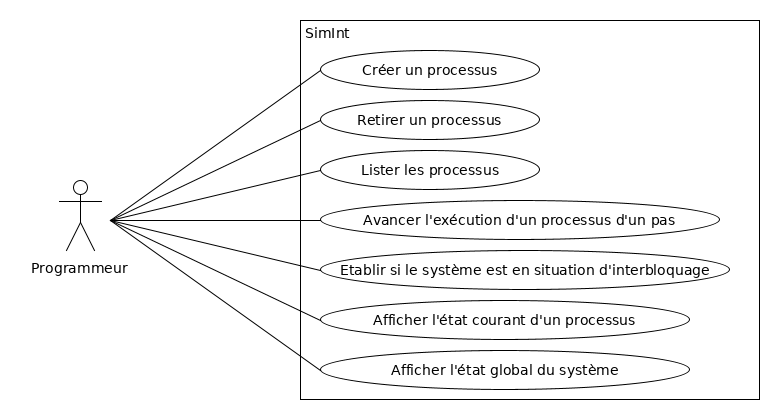
\includegraphics[scale=0.5]{DiagrammesDeCasDUtilisation/simint_uml_diag_cas_utilisation_processus}
\caption{Diagramme de cas d'utilisation}
\end{center}
\label{usecase_umlet_simint}
\end{figure}

\newpage

\subsection{Priorités, préconditions et postconditions des cas d'utilisation}

Les priorités des cas d'utilisation pour le sprint~1 sont choisies
avec les règles de bon sens suivantes:
\begin{compactitem}
\item pour retirer une entité du système, elle doit y être. La
priorité de l'ajout est donc supérieure ou égale à la priorité du
retrait;
\item pour lister les entités d'un type donné, elles doivent y être. La
priorité de l'ajout est donc supérieure ou égale à la priorité du
listage;
\item il est \textit{a priori} possible, c.-à-d. sans raison
contraire, de démontrer la mise en œuvre d'un sous-ensemble des
fonctionnalités du système, et plus particulièrement la prise en
compte des principales règles de gestion, sans les retraits ou les
listages.
\item la possibilité de lister aide au déverminage de l'application
pendant les activités d'exécution des tests de validation.
\end{compactitem}
Par conséquent, les cas d'utilisation d'ajout sont \textit{a priori}
de priorité <<~haute~>>, ceux de listage de priorité <<~moyenne~>>, et
ceux de retrait de priorité <<~basse~>>.

\bigskip

Dans la suite, nous donnons les préconditions et postconditions pour
les cas d'utilisation de priorité <<~\haute~>>. Pour les autres, nous
indiquons uniquement leur niveau de priorité.

\bigskip

{\color{red}\textbf{La précondition suivante est à compléter.}}

\begin{compactitem}
\usecase{\haute}{Créer un processus}
{nom de processus bien formé (non \nullvalue et non vide) $\land$
processus avec ce nom inexistant $\land$ exécution non débutée}
{processus avec ce nom}

\smallskip

\priorityusecase{\basse}{Retirer un processus}

\smallskip

\priorityusecase{\moyenne}{Lister les processus}
\end{compactitem}

\newpage

\section{Préparation des tests de validation}

\subsection{Tables de décision des tests de validation}

La fiche programme du module CSC4102 ne permettant pas de développer
des tests de validation couvrant l'ensemble des cas d'utilisation de
l'application, les cas d'utilisation choisis sont de priorité
\textsc{Haute}.

{\color{red}\textbf{La table de décision suivante est à compléter.}}

\begin{table}[htbp!]
\begin{tabular}{|p{0.6\linewidth}|c|c|c|c|}
\hline
Numéro de test
&1&2&3&4\\
\hline
\hline
Nom processus bien formé ($\neq$ \nullvalue $\land$ $\neq$ vide)
&F&T&T&T\\
\hline
Exécution non débutée
& &F&T&T\\
\hline
Processus inexistant avec ce nom
& & &F&T\\
\hline
\hline
Création acceptée
&F&F&F&T\\
\hline
\hline
Nombre de jeux de test 
&2&1&1&1\\
\hline
\end{tabular}
\caption{Cas d'utilisation <<~créer un processus~>>}
\end{table}

\newpage

\section{Conception}

\subsection{Liste des classes}

{\color{red}\textbf{La liste des classes suivante est à compléter.}}

À la suite d'un parcours des diagrammes de cas d'utilisation et d'une
relecture de l'étude de cas, voici une première liste de classes avec
quelques attributs:
\begin{compactitem}
\item \textsf{SimInt} (la façade),
\item \textsf{Processus}~---~nom,
\item \textsf{ÉtatGlobal} (l'état du système)~---~,
\item \textsf{ÉtatProcessus} (la partie de l'état concernant les processus)~---~.
\end{compactitem}
\newpage

\subsection{Diagramme de classes}

{\color{red}\textbf{Le diagramme de classes suivant est à compléter.}}

\begin{figure}[h!]
\begin{center}
\includegraphics[scale=0.6]{DiagrammesDeClasses/simint_uml_diag_classes_elementsdedepart}
\caption{Diagramme de classes}
\end{center}
\label{umlet_diag_classes}
\end{figure}

\newpage

\subsection{Diagramme d'objets}

Comme l'une des difficultés de l'étude de cas est de comprendre, pour
l'utiliser, la copie légère et la copie profonde, nous dessinons un
diagramme d'objets de deux états globaux.

{\color{red}\textbf{Le diagramme d'objets suivant est à compléter.}}

\begin{figure}[h!]
%% \begin{center}
\hspace{-1cm}\includegraphics[scale=0.5]{DiagrammesDObjets/simint_uml_diag_objets}
\caption{Diagramme d'objets à partir de l'état initial}
%% \end{center}
\label{umlet_diag_classes}
\end{figure}

\newpage

\subsection{Diagrammes de séquence}

{\color{red}\textbf{La description et le diagramme de séquence suivants sont à compléter.}}

Voici la description textuelle du cas d'utilisation <<~créer un processus~>>:
\begin{compactitem}
\item arguments en entrée: nom du processus, nom du programme
\item rappel de la précondition: nom du processus bien formé (non
  \nullvalue et non vide) $\land$ processus avec ce nom existant
  $\land$ exécution non débutée
\item algorithme:
  \begin{compactenum}
  \item vérifier les arguments
  \item si en outre l'exécution du système n'a pas débuté
    \begin{compactenum}
    \item vérifier que le processus n'existe pas
    \item créer un processus avec ce nom
    \item ajouter le processus à la collection des processus
    \item ajouter un état dans l'état global initial pour ce processus
    \begin{compactenum}
    \item créer un état pour ce processus
    \item ajouter l'état de processus à l'état global initial
    \end{compactenum}
    \end{compactenum}
  \end{compactenum}
\end{compactitem}

\begin{figure}[ht!]
\begin{center}
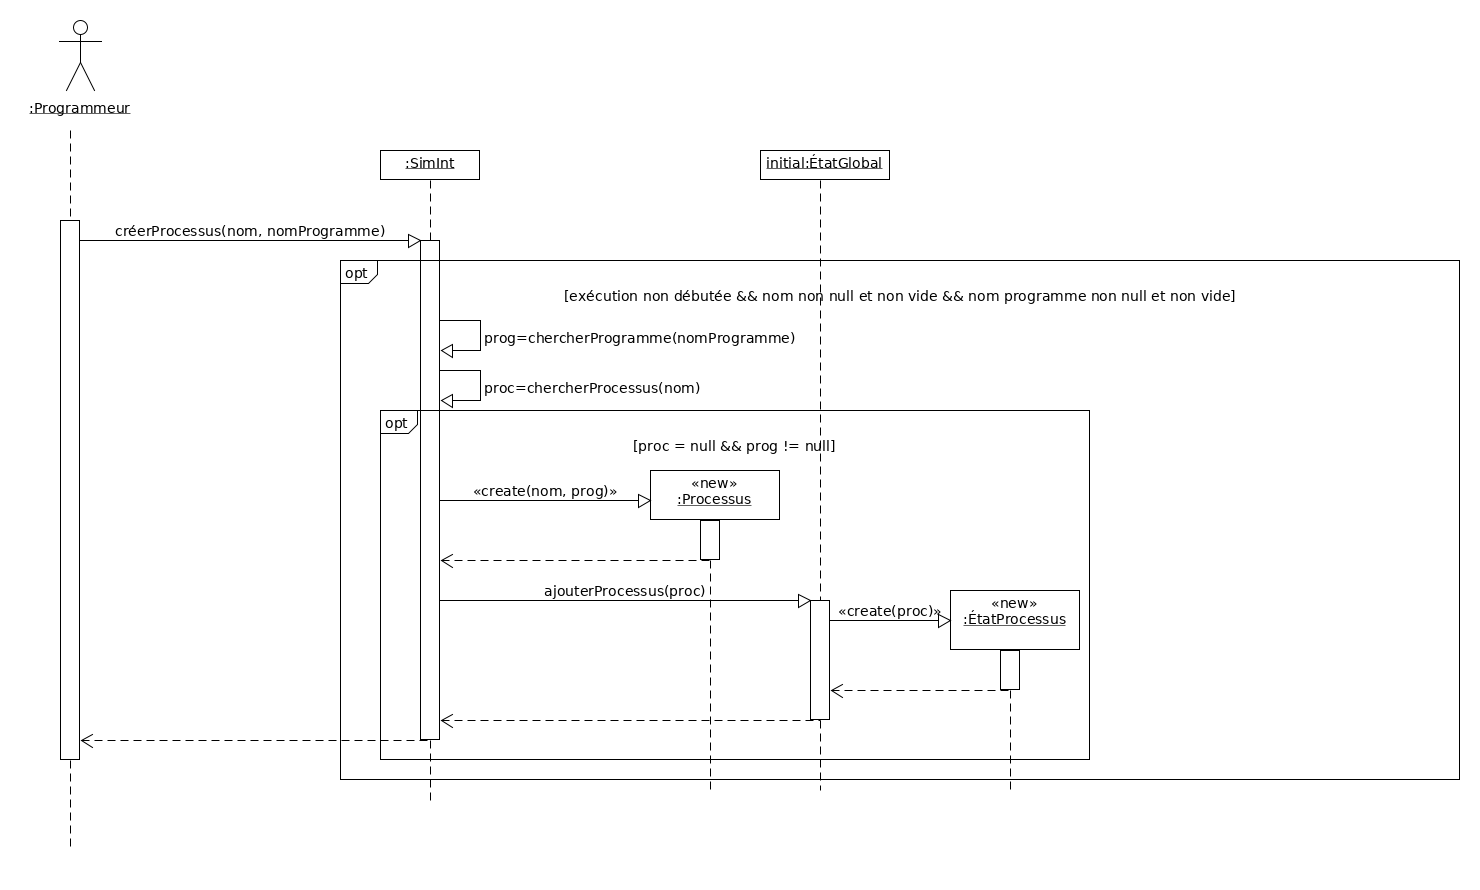
\includegraphics[scale=0.48]{DiagrammesDeSequence/simint_uml_diag_sequence_creer_processus}
\caption{Diagramme de séquence du cas d'utilisation <<~créer un processus~>>}
\end{center}
\label{umlet_diag_sequence_creer_processus}
\end{figure}

\newpage

\section{Fiche des classes}

{\color{red}\textbf{Les fiches des classes suivantes sont à compléter.}}

\subsection{Classe \textsf{SimInt}}

\begin{center}
\begin{longtable}{|p{15cm}|} 
\hline
\multicolumn{1}{|c|}{{\Large \textsf{Simint}}} \\
\hline
%\cmt{attributs}\\
\cmt{attributs <<~association~>>}\\
$-$ processus : collection de @Processus \\
$-$ étatGlobalInitial : ÉtatGlobal \\
$-$ exécutionDébutée : booléen \\
\hline
\cmt{constructeur} \\
$+$ SimInt()\\
\cmt{operations <<~cas d'utilisation~>>} \\
$+$ créerProcessus(String nom) \\
$+$ chercherProcessus(String nom) : Processus \\
\hline  
\end{longtable}%)
\end{center}

\newpage

\subsection{Classe \textsf{Processus}}

\begin{center}
\begin{longtable}{|p{15cm}|} 
\hline
\multicolumn{1}{|c|}{{\Large \textsf{Processus}}} \\
\hline
\cmt{attributs}\\
$-$ nom : String \\
%% \cmt{attributs <<~association~>>}\\
\hline
\cmt{constructeur} \\
$+$ constructeurProcessus(String nom)\\
%% \cmt{operations <<~cas d'utilisation~>>} \\
%% \cmt{opérations de recherche} \\
\hline  
\end{longtable}%)
\end{center}

\subsection{Classe \textsf{ÉtatProcessus}}

\begin{center}
\begin{longtable}{|p{15cm}|} 
\hline
\multicolumn{1}{|c|}{{\Large \textsf{ÉtatProcessus}}} \\
\hline
\cmt{attributs}\\
$-$ processus : Processus \\
\underline{$-$ compteurInstanciation : entier = 0} \\
$-$ compteurInstance : entier \\
%% \cmt{attributs <<~association~>>}\\
\hline
\cmt{constructeur} \\
$+$ constructeurProcessus(Processus processus)\\
$+$ constructeurProcessus(ÉtatProcessus étatProcessus) // constructeur par copie\\
%% \cmt{operations <<~cas d'utilisation~>>} \\
%% \cmt{opérations de recherche} \\
\hline  
\end{longtable}%)
\end{center}

\newpage

\subsection{Classe \textsf{ÉtatGlobal}}

\begin{center}
\begin{longtable}{|p{15cm}|} 
\hline
\multicolumn{1}{|c|}{{\Large \textsf{ÉtatGlobal}}} \\
\hline
\cmt{attributs}\\
$-$ estÉtatGlobalInitial : booléen \\
$-$ étatsGlobauxAtteignables : collection de @ÉtatGlobal \\
\underline{$-$ compteurInstanciation : entier = 0} \\
$-$ compteurInstance : entier \\
\cmt{attributs <<~association~>>}\\
$-$ étatsProcessus : collection ordonnée de @ÉtatProcessus \\
\hline
\cmt{constructeurs} \\
$+$ constructeurÉtatGlobal()\\
$+$ constructeurÉtatGlobal(ÉtatGlobal origine) // constructeur par copie\\
\cmt{operations <<~cas d'utilisation~>>} \\
$+$ ajouteÉtatProcessus(Processus processus) \\
$+$ chercherÉtatProcessus(String nom) : @ÉtatProcessus \\
\hline  
\end{longtable}%)
\end{center}

\newpage

\section{Diagrammes de machine à états et invariants}

{\color{red}\textbf{Les invariants suivants sont à compléter.}}

\subsection{Classes \textsf{Processus}}

L'invariant de la classe \textsf{Processus} est le suivant:
\newcommand{\nom}{\ensuremath\mathrm{nom}}
\newcommand{\vvide}{\ensuremath\mathrm{``"}}
\begin{tabbing}
M \= M \= M \= M \= M \= M \= M \kill
\> $\nom \neq \nullvalue \land \nom \neq \vvide$\\
\end{tabbing}

\subsection{Classes \textsf{ÉtatProcessus}}

\newcommand{\processus}{\ensuremath\mathrm{processus}}
L'invariant de la classe \textsf{ÉtatProcessus} est le suivant:
\begin{tabbing}
M \= M \= M \= M \= M \= M \= M \kill
\> $\processus \neq \nullvalue$\\
\end{tabbing}

\subsection{Classes \textsf{ÉtatGlobal}}

\newcommand{\etatsprocessus}{\ensuremath\mathrm{etatsProcessus}}
L'invariant de la classe \textsf{ÉtatGlobal} est le suivant:
\begin{tabbing}
M \= M \= M \= M \= M \= M \= M \kill
\> $\etatsprocessus \neq \nullvalue$\\
\end{tabbing}

\newpage

\section{Préparation des tests unitaires}

\subsection{Classe \textsf{Processus}}

\begin{table}[h!]
\begin{center}
\begin{tabular}{|p{0.6\linewidth}|c|c|}
\hline
Numéro de test
&1&2\\
\hline
\hline
\texttt{nom} $\neq \nullvalue \land \neg \emptyvalue$
&F&T\\
\hline
\hline
$\nom' \neq \nullvalue \land \neg \emptyvalue$
& &T\\
\hline
$\invariant$
& &T\\
\hline
Levée d'une exception&\textsc{oui}&\textsc{non}\\
\hline
\hline
Objet créé
&F&T\\
\hline
\hline
Nombre de jeux de test 
&2&1\\
\hline
\end{tabular}
\caption{Méthode \texttt{constructeurProcessus} de la
classe \texttt{Processus}~>>}
\end{center}
\end{table}

\newpage

\pagenumbering{arabic}
\renewcommand*{\thepage}{\roman{page}}

\appendix

\section{Algorithmes des classes}

{\color{red}\textbf{Les algorithmes des classes suivantes sont à compléter.}}

\subsection{Classe \textsf{SimInt}}

\begin{tabbing}
MMM \= MMM \= MMM \= MMM \= MMM \kill
\rule{12cm}{0.2mm} \\
\textsf{\large constructeurSimint()} \\
\> processus = nouvelle collection vide\\
\> étatGlobalInitial = constructeurÉtatGlobal()\\
\> exécutionDébutée = false\\
\rule{12cm}{0.2mm}
\end{tabbing}

\begin{tabbing}
MMM \= MMM \= MMM \= MMM \= MMM \kill
\rule{12cm}{0.2mm} \\
\textsf{\large créerProcessus(String nom)} \\
\> si (nom null OU nom chaîne vide)\\
\> \> lever exception\\
\> si exécution déjà débutée \\
\> \> lever exception \\
\> Processus proc = chercherProcessus(nom)\\
\> si (proc = null) \\
\> \> proc = constructeurProcessus(nom, p)\\
\> \> étatInitial.ajouterProcessus(proc)\\
\rule{12cm}{0.2mm}
\end{tabbing}

\newpage

\subsection{Classe \textsf{Processus}}

\begin{tabbing}
MMM \= MMM \= MMM \= MMM \= MMM \kill
\rule{12cm}{0.2mm} \\
\textsf{\large constructeurProcessus(String nom)} \\
\> si (nom null OU nom chaîne vide) // programmation défensive\\
\> \> lever exception\\
\> this.nom = nom\\
\> assert invariant()\\
\rule{12cm}{0.2mm}
\end{tabbing}

\subsection{Classe \textsf{ÉtatProcessus}}

\begin{tabbing}
MMM \= MMM \= MMM \= MMM \= MMM \kill
\rule{12cm}{0.2mm} \\
\textsf{\large constructeurProcessus(Processus processus)} \\
\> si (processus = null)\\
\> \> lever exception\\
\> this.processus = processus\\
\> compteurInstanciation++\\
\> compteurInstance = compteurInstanciation\\
\> assert invariant()\\
\rule{12cm}{0.2mm}
\end{tabbing}

\begin{tabbing}
MMM \= MMM \= MMM \= MMM \= MMM \kill
\rule{12cm}{0.2mm} \\
\textsf{\large constructeurProcessus(ÉtatProcessus étatProcessus)} \\
\> si (étatProcessus = null)\\
\> \> lever exception\\
\> this.processus = proc.processus\\
\> compteurInstanciation++\\
\> compteurInstance = compteurInstanciation\\
\> assert invariant()\\
\rule{12cm}{0.2mm}
\end{tabbing}

\newpage

\subsection{Classe \textsf{ÉtatGlobal}}

\begin{tabbing}
MMM \= MMM \= MMM \= MMM \= MMM \kill
\rule{12cm}{0.2mm} \\
\textsf{\large constructeurÉtatGlobal()} \\
\> étatGlobalInitial = true\\
\> étatsProcessus = création d'une collection vide\\
\> étatsGlobauxAtteignables = création d'une collection vide\\
\> compteurInstanciation++\\
\> compteurInstance = compteurInstanciation\\
\> assert invariant()\\
\rule{12cm}{0.2mm}
\end{tabbing}

\begin{tabbing}
MMM \= MMM \= MMM \= MMM \= MMM \kill
\rule{12cm}{0.2mm} \\
\textsf{\large constructeurÉtatGlobal(ÉtatGlobal origine)} \\
\> étatGlobalInitial = false\\
\> étatsProcessus = copie légère de la collection origine.étatsProcessus\\
\> étatsGlobauxAtteignables = création d'une collection vide\\
\> compteurInstanciation++\\
\> compteurInstance = compteurInstanciation\\
\> assert invariant()\\
\rule{12cm}{0.2mm}
\end{tabbing}

\begin{tabbing}
MMM \= MMM \= MMM \= MMM \= MMM \kill
\rule{12cm}{0.2mm} \\
\textsf{\large ajouteProcessus(Processus processus)} \\
\> si (!étatInitial) // programmation défensive\\
\> \> lever exception\\
\> si (processus = null) // programmation défensive\\
\> \> lever exception\\
\> étatProcessus = constructeurÉtatProcessus(processus)\\
\> si (étatsProcessus contient déjà étatProcessus)\\
\> \> lever exception\\
\> ajouter étatProcessus à la collection étatsProcessus\\
\> assert invariant()\\
\rule{12cm}{0.2mm}
\end{tabbing}

\end{document}
